\documentclass[aspectratio=169]{beamer}

%%% TEMA
\usetheme[progressbar=frametitle]{metropolis}
\usecolortheme{beaver}
\useinnertheme{metropolis}
\useoutertheme{metropolis}
\usefonttheme{metropolis}
\setbeamercolor{background canvas}{bg=white}

%%% PACCHETTI
\usepackage{graphicx}
\usepackage[italian]{babel}
\usepackage[utf8]{inputenc}
\usepackage{subcaption}
\usepackage{media9}

%%% DATI
\author{\textbf{Cristian Mercadante}}
\title[Installazione e Configurazione di ShareLaTeX]{Installazione e Configurazione di\\ShareLaTeX su Piattaforma Docker}
\institute{\small
\textbf{Relatore:}\\
Prof. Costantino Grana\\
\textbf{Correlatore:}\\
Dott. Federico Bolelli
}
\date{}


\begin{document}

\begin{frame}
    \titlepage
\end{frame}

\begin{frame}{ShareLaTeX}
    \begin{center}
        
\includegraphics[scale=0.25]{img/sharelatex_logo.png}
    \end{center}
    \begin{columns}[T]
        \begin{column}{0.5\textwidth}
            \textbf{Cos'è}
            \begin{itemize}
                \item Applicazione web
                \item Editor \LaTeX
                \item Compilatore \LaTeX
                \item Archivio di progetti online
            \end{itemize}
        \end{column}
        \begin{column}{0.5\textwidth}
            \textbf{Funzionalità}
            \begin{itemize}
                \item Condivisione dei progetti
                \item Collaborazione in scrittura
                \item Conservazione dello storico delle modifiche
            \end{itemize}
        \end{column}
    \end{columns}
\end{frame}

\begin{frame}{Motivazioni e obiettivi}
    \begin{center}
        \vspace{-1.5cm}
        
\includegraphics[scale=1.5]{img/aimagelab_logo.png}
    \end{center}
    \vspace{-1.5cm}
    \begin{columns}[T]
        \begin{column}{0.5\textwidth}
            \textbf{Motivazioni}
            \begin{itemize}
                \item Evitare disconnessione
                \item Progetti salvati sul server del dipartimento
            \end{itemize}
        \end{column}
        \begin{column}{0.5\textwidth}
            \textbf{Obiettivi}
            \begin{itemize}
                \item Installazione di ShareLaTeX
                \item Facile manutenzione
            \end{itemize}
        \end{column}
    \end{columns}
\end{frame}

\begin{frame}{Docker}
    \begin{center}
        
\includegraphics[scale=0.13]{img/docker_logo_2.png}
    \end{center}
    \begin{columns}[T]
        \begin{column}{0.333\textwidth}
            \textbf{Cos'è}
            \begin{itemize}
                \item Piattaforma per sviluppo e consegna di applicazioni
                \item Creatore di \emph{container}
            \end{itemize}
        \end{column}
        \begin{column}{0.333\textwidth}
            \textbf{Funzionalità}
            \begin{itemize}
                \item Esecuzione di applicazioni in ambienti protetti
                \item Portabilità e scalabilità
                \item Performance migliori rispetto alle VMs
             \end{itemize}
        \end{column}
        \begin{column}{0.333\textwidth}
            \textbf{Componenti principali}
            \begin{itemize}
                \item Docker Engine
                \item Docker Hub
            \end{itemize}
        \end{column}
    \end{columns}
\end{frame}

\begin{frame}{Containers VS Virtual Machines}
    \begin{center}
        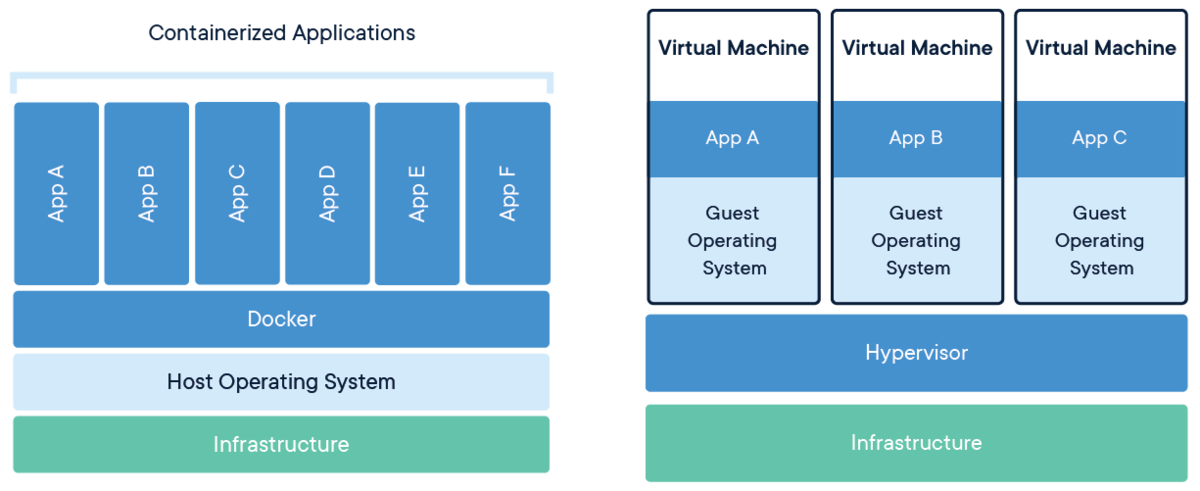
\includegraphics[width=\textwidth]{img/docker-containerized-and-vm-transparent-bg.png}
    \end{center}
\end{frame}

\begin{frame}{Componenti e tool}
    \begin{columns}[T]
        \begin{column}{0.25\textwidth}
            
\includegraphics[width=\textwidth]{img/mongodb_logo.jpg}
        \end{column}
        \begin{column}{0.25\textwidth}
            
\includegraphics[width=\textwidth]{img/redis_logo.png}
        \end{column}
        \begin{column}{0.25\textwidth}
            \vspace{0.10cm}
            
\includegraphics[width=\textwidth]{img/nginx_logo.png}
        \end{column}
        \begin{column}{0.25\textwidth}
            \vspace{-0.5cm}
            
\includegraphics[width=\textwidth]{img/docker_compose_logo.png}
            \vspace{0.5cm}
        \end{column}
    \end{columns}
    \begin{columns}[T]
        \begin{column}{0.25\textwidth}
            \begin{itemize}
                \item Database NoSQL
                \item Database centrale per ShareLaTeX
            \end{itemize}
        \end{column}
        \begin{column}{0.25\textwidth}
            \begin{itemize}
                \item Database NoSQL
                \item Meccanismo di caching per ShareLaTeX
            \end{itemize}
        \end{column}
        \begin{column}{0.25\textwidth}
            \begin{itemize}
                \item Web server
                \item Utilizzato come reverse-proxy per certificati HTTPS
            \end{itemize}
        \end{column}
        \begin{column}{0.25\textwidth}
            \begin{itemize}
                \item Estensione di Docker
                \item Strumento per l'esecuzione di servizi multicontainer
            \end{itemize}
        \end{column}
    \end{columns}
\end{frame}

\begin{frame}{Architettura}
    \vspace{0.5cm}
    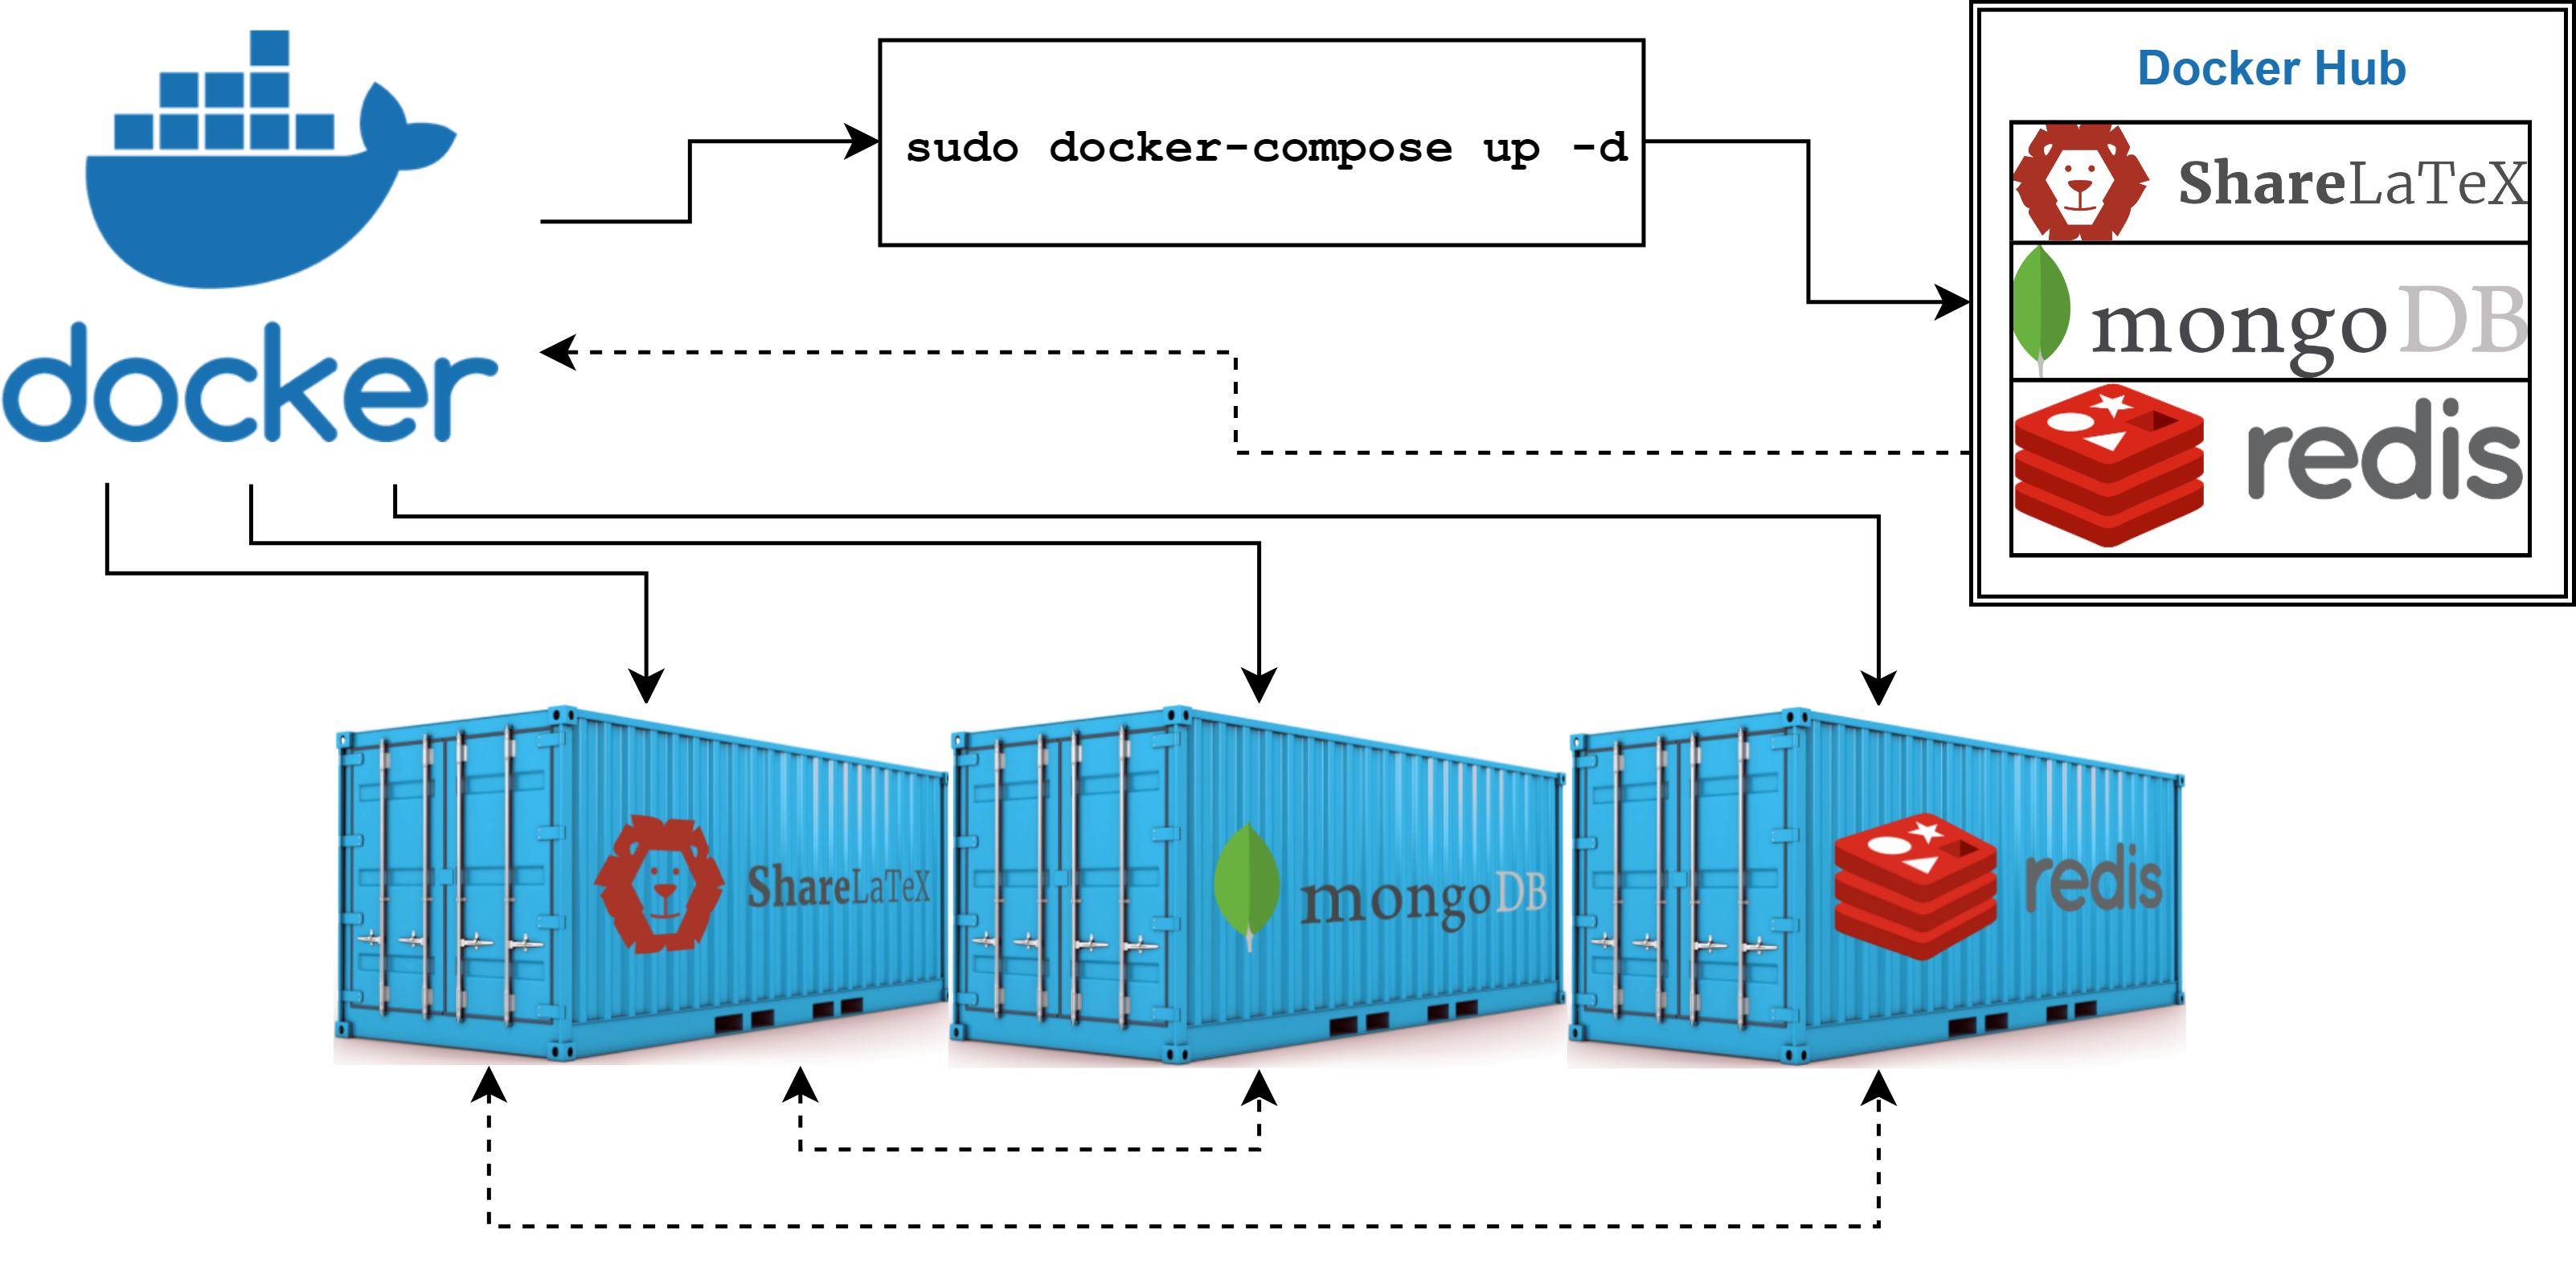
\includegraphics[width=\textwidth]{img/docker_container_dependencies.png}
\end{frame}

\begin{frame}{Fasi}
    \begin{columns}[T]
        \begin{column}{0.333\textwidth}
            \textbf{Installazione}
            \begin{enumerate}
                \item Docker
                \item Docker Compose
                \item Pacchetti TeX Live
                \item NGINX reverse-proxy per HTTPS
            \end{enumerate}
       \end{column}
       \begin{column}{0.333\textwidth}
            \textbf{Configurazione}
            \begin{enumerate}\setcounter{enumi}{4}
                \item Utente amministratore
                \item Interfaccia
                \item Mail SMTP
            \end{enumerate}
       \end{column}
       \begin{column}{0.333\textwidth}
            \textbf{Manutenzione}
            \begin{enumerate}\setcounter{enumi}{7}
                \item Backup dei container
                \item Ripristino del sistema
                \item Script di aggiornamento del sistema
            \end{enumerate}
       \end{column}
    \end{columns}
\end{frame}

\begin{frame}{Dimostrazione}

\includemedia[
    width=\textwidth,
    height=\textheight-0.5cm,
    keepaspectratio,
    addresource=demo.mp4,
    transparent,
    playbutton=plain,
    activate=onclick,
    flashvars={
        source=demo.mp4
        &autoPlay=true
        &loop=false
    }
]{
\includegraphics[]{img/sharelatex_demo.png}}{VPlayer9.swf}
    
\end{frame}

\begin{frame}{}
\centering
\Huge
Grazie per l'attenzione
\end{frame}

\end{document}